\documentclass{article}
\usepackage[english]{babel}
\usepackage{mathtools}
\usepackage{graphicx}

\title{Backwards algorithm for coverability exercise}
\author{Adrián Enríquez Ballester}

\begin{document}
\maketitle

Apply the backwards reachability algorithm to the Petri net 
below to decide if the marking $M = (0, 0, 2)$ can be covered.

\begin{center}
  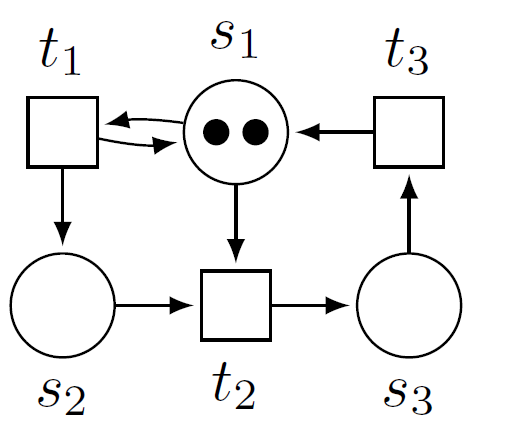
\includegraphics[scale=0.4]{net}
\end{center}

Record all intermediate steps and all the intermediate sets of 
markings with their finite representation of minimal elements.

\section*{Answer}

\subsection*{Preliminaries}

First of all, let us gather the minimal markings that allow us 
to fire ``backwards'' the transitions of the net:

$$R[t_1] = (1, 1, 0)$$
$$R[t_2] = (0, 0, 1)$$
$$R[t_3] = (1, 0, 0)$$

We are going to annotate with a subindex the variable $m$ 
of the algorithm for specifying its corresponding iteration, 
so the initial one is

$$m_0 \coloneqq \{ (0, 0, 2) \}$$

and the sequence is computed iteratively with the following 
termination conditions, being $i$ the current one in 
the algorithm execution:

\begin{enumerate}
  \item Some marking from $m_i$ is smaller or equal than $M_0$, 
    which means that $M$ can be covered.
  \item The sequence stabilizes (i.e. $m_i = m_{i - 1}$) and the 
  previous condition does not hold, which means that $M$ cannot be covered.
\end{enumerate}

Note also that $M_0 = (2, 0, 0)$ is the initial marking. 

\subsection*{Iteration $i$ explanation}

Each iteration computes 

$$
  m_i = m_{i - 1} \cup 
    \Big(
      \bigcup\limits_{t \in T} pre(R[t] \land m_{i - 1}, t)
    \Big)
$$

where $T = \{ t_1, t_2, t_3 \}$. For that, it also needs to compute
$pre(R[t] \land m_{i - 1}, t)$, which also requires  
$R[t] \land m_{i - 1}$.

All these finite representations of marking sets are shown for 
each iteration, alongside with a small comment about its termination 
check.

\subsection*{Iteration 1}

$$R[t_1] \land m_0 = \{ (1, 1, 2) \}$$
$$R[t_2] \land m_0 = \{ (0, 0, 2) \}$$
$$R[t_3] \land m_0 = \{ (1, 0, 2) \}$$

$$pre(R[t_1] \land m_0, t_1) = \{ (1, 0, 2) \}$$
$$pre(R[t_2] \land m_0, t_2) = \{ (1, 1, 1) \}$$
$$pre(R[t_3] \land m_0, t_3) = \{ (0, 0, 3) \}$$

$$m_1 \coloneqq \{ (0, 0, 2), (1, 1, 1) \}$$

As none of $(0, 0, 2)$ and $(1, 1, 1)$ is smaller or equal than 
$M_0$ and $m_0 \neq m_1$, we proceed to the next iteration.

\subsection*{Iteration 2}

$$R[t_1] \land m_1 = \{ (1, 1, 1) \}$$
$$R[t_2] \land m_1 = \{ (0, 0, 2), (1, 1, 1) \}$$
$$R[t_3] \land m_1 = \{ (1, 0, 2), (1, 1, 1) \}$$

$$pre(R[t_1] \land m_1, t_1) = \{ (1, 0, 1) \}$$
$$pre(R[t_2] \land m_1, t_2) = \{ (1, 1, 1), (2, 2, 0) \}$$
$$pre(R[t_3] \land m_1, t_3) = \{ (0, 0, 3), (0, 1, 2) \}$$

$$m_2 \coloneqq \{ (0, 0, 2), (1, 0, 1), (2, 2, 0) \}$$

Again, as none of $(0, 0, 2), (1, 0, 1)$ and $(2, 2, 0)$ is 
smaller or equal than $M_0$ and $m_1 \neq m_2$, we proceed to the 
next iteration.

\subsection*{Iteration 3}

$$R[t_1] \land m_2 = \{ (1, 1, 1), (2, 2, 0) \}$$
$$R[t_2] \land m_2 = \{ (0, 0, 2), (1, 0, 1) \}$$
$$R[t_3] \land m_2 = \{ (1, 0, 1), (2, 2, 0) \}$$

$$pre(R[t_1] \land m_2, t_1) = \{ (1, 0, 1), (2, 1, 0) \}$$
$$pre(R[t_2] \land m_2, t_2) = \{ (1, 1, 1), (2, 1, 0) \}$$
$$pre(R[t_3] \land m_2, t_3) = \{ (0, 0, 2), (1, 2, 1) \}$$

$$m_3 \coloneqq \{ (0, 0, 2), (1, 0, 1), (2, 1, 0) \}$$

Again, as none of $(0, 0, 2), (1, 0, 1)$ and $(2, 1, 0)$ is 
smaller or equal than $M_0$ and $m_2 \neq m_3$, we proceed to the 
next iteration.

\subsection*{Iteration 4}

$$R[t_1] \land m_3 = \{ (1, 1, 1), (2, 1, 0) \}$$
$$R[t_2] \land m_3 = \{ (0, 0, 2), (1, 0, 1) \}$$
$$R[t_3] \land m_3 = \{ (1, 0, 1), (2, 1, 0) \}$$

$$pre(R[t_1] \land m_3, t_1) = \{ (1, 0, 1), (2, 0, 0) \}$$
$$pre(R[t_2] \land m_3, t_2) = \{ (1, 1, 1), (2, 1, 0) \}$$
$$pre(R[t_3] \land m_3, t_3) = \{ (0, 0, 2), (1, 1, 1) \}$$

$$m_4 \coloneqq \{ (0, 0, 2), (1, 0, 1), (2, 0, 0) \}$$

Finally, as $(2, 0, 0)$ in $m_4$ is precisely $M_0$, we have 
that $M_0$ belongs to $pre^{*}(M\uparrow)$, thus $M$ can 
be covered.

\end{document}
